\section{Transition metal dichalcogenides and WS$_2$}
\label{sec:tmd}

In this work we will apply our machine learning-based method
for describing the ZLP to a novel class of tungsten disulfide (WS$_2$) nanostructures known
as nanoflowers~\cite{SabryaWS2}.

WS$_2$ is a transition metal dichalcogenide (TMD) material, which 
belongs to a large family of materials known as 2D materials or van der Waals materials.
%
They are named two-dimensional to emphasize their extraordinary thinness: 
TMDs are characterised by the remarkable property of being fully 
functional down to a single atomic layer.
%
A monolayer MoS$_2$ is only 6.5 Å thick. 
%
Just like graphite is a stacking of individual layers of graphene,
bulk crystals can be formed by stacking 2D monolayers, 
 bound to each other by Van der Waals attraction. 
%
Over the past few years the exploration of these 2D layered materials
 has developed rapidly. 
 %
 In particular significant attention has been 
 going to monolayers of transition metal dichalcogenides,
 atomically thin semiconductor of the type $MX_2$, here M is a 
transition metal atom (such as Mo or W) and X is a chalcogen atom (such as S, Se, or Te). 
 %
The characteristic crystalline structure of TMDs is one layer of M atoms 
that is sandwiched between two layers of X atoms.
 %
The electronic structure of TMDs strongly depends on the coordination 
 of the transition metal atoms, giving rise to a variety of electronic
 and magnetic properties~\cite{Chhowalla:2013}.
 %
In fact, most of the remarkable electronic and optical properties of TMDs
can be traced back to the underlying periodic arrangements of their layers, 
the so-called stacking sequences~\cite{SabryaWS2}.
%
Furthermore, the properties of this class of materials vary significantly
with their thickness, for instance MoS$_2$ exhibits an indirect bandgap
in the bulk form which becomes direct at the monolayer level~\cite{Splendiani:2010}.
%
The indirect-to-direct bandgap transition is the main reason for the interest in 
the use of TMDs for flexible electronics: it emphasizes the importance of the
mechanical properties of these materials. 
%
However, it tends to be much more difficult to uniformly deform 2D monolayers
of a material compared to bulk samples, and therefore measuring on 2D systems
can be challenging.
%
TMDs are often combined with other 2D materials like graphene
to make Van der Waals heterostructures, which need to be tuned in order
to function as building blocks for many devices such as LEDs, solar cells, 
transistors, and photodetectors.
%
This research field is still emerging and highly promosing to have a big
impact on future nanotechnology. \\
 
An example of a TMD exhibiting a pronounced dependence on its thickness is 
thungsten disulfide (WS$_2$), with an indirect-to-direct bandgap transition when going
from bulk to bilayer or monolayer form.
%
The effects of this transition are manifested as enhanced
photoluminescence in monolayer WS$_2$, whereas only little emission is observed in
the corresponding bulk form.
%
WS$_2$ adopts a layered structure by stacking atomic layers of S-W-S 
in a sandwich-like configuration. 
%
Although the interaction between adjacent layers is a weak Van der Waals 
force, the dependence of the interlayer interaction on the stacking 
order of WS$_2$ is significant.
%
Further applications of this material include storage of hydrogen 
and lithium for batteries~\cite{Bhandavat:2012}.

%%%%%%%%%%%%%%%%%%%%%%%%%%%%%%%%%%%%%%%%%%%%%%%%%%%%%%%%%%%%%%%%%%%%%%%%%%%%%%%
\begin{figure}[h]
    \centering
    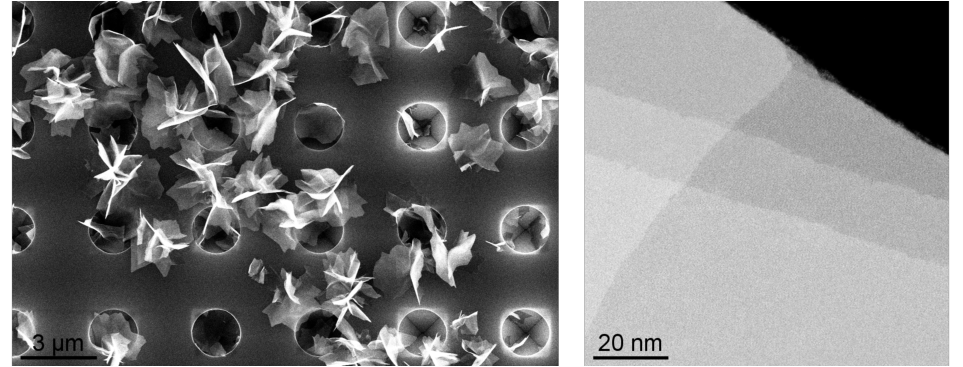
\includegraphics[width=0.8\textwidth]{plots/spectrumimage.pdf}
    \caption{Left: low-magnification TEM image of WS$_2$ nanoflowers
      grown on top of a porous TEM substrate. Right: the magnification of a representative 
      petal of a nanoflower, where the black region corresponds to 
      the vacuum (no substrate) and the difference in contrast indicates terraces of varying thickness.}
    \label{fig:nanoflowers}
\end{figure}
%%%%%%%%%%%%%%%%%%%%%%%%%%%%%%%%%%%%%%%%%%%%%%%%%%%%%%%%%%%%%%%%%%%%%%%%%%%%%%%%%%5

A low-magnification TEM image of the WS$_2$ nanoflowers presented in~\cite{SabryaWS2} is displayed
in the left panel of Fig.~\ref{fig:nanoflowers}.
%
These nanostructures are grown directly on top of a TEM substrate with holes in it. 
%
The right panel shows the magnification of a representative petal of a nanoflower,
where the difference in contrast indicates terraces of varying thickness.
%
Note that the black region corresponds to the vacuum, without
substrate underneath.
%
These WS$_2$ nanoflowers contain areas with different thicknesses, orientations
and crystalline structures, therefore representing an ideal environment to investigate
structural morphology in WS$_2$ with electronic properties at the nanoscale.
%
What makes it even more interesting is that these nanoflowers display 3R/2H polytypism, 
an important issue for the interlayer
 interactions within WS$_2$: different stacking types tend to coexist, 
 complicating the characterization of the physical properties~\cite{Na:2018}.
%
One possible response of polytypism to electric fields is
 spontaneous electrical polarization, leading to modifications on the 
 electronic band structure and correspondingly on the band gap.
 %
Tailoring the specific stacking sequences (polytypes) 
represents a powerful strategy to identify and design novel physical properties~\cite{SabryaWS2}.
%

As mentioned before, one of the most interesting properties of TMDs that also
occurs in WS$_2$ is the fact when the material
is thinned down to a single monolayer, its indirect band gap of
$E_{\rm bg}\simeq 1.4$ eV
switches to a direct band gap of approximately $E_{\rm bg}\simeq 2.1$ eV.
%
In general, it has been found that the type and magnitude of the bandgap
of WS$_2$ depends quite sensitively on the crystalline structure and
the number of layers that constitute the material.
%
In Table~\ref{table:bgvalues} we collect
representative results for the determination of the bandgap energy $E_{\rm bg}$
and its type in WS$_2$, obtained by means of different experimental and theoretical techniques.
%
For each reference we indicate separately the bulk results and those
obtained at the monolayer level.
%
We observe that for monolayers, the results for the measured
value of $E_{\rm bg}$ are quite inconsistent, 
reflecting the challenges of its accurate determination.


 
%%%%%%%%%%%%%%%%%%%%%%%%%%%%%%%%%%%%%%%%%%%%%%%%%%%%%%%%%%%%%%%%%%%%%%%%%%%%%%%%%%%%%
\begin{table}[H]
  \small
  \begin{centering}
   \renewcommand{\arraystretch}{1.20}
\begin{tabular}{ccccc}
\br
Reference                       & Thickness & $E_{\rm bg}$ (eV)  & Band gap type  & Technique \\
\mr
{\cite{Braga:2012}} & bulk   & $1.4\pm0.07$            & indirect  & {Gate-voltage dependence}  \\
\mr
\multirow{}{}{\cite{Jo:2014}}                 & ML   & $2.14 $         & direct  & \multirow{}{}{Gate-voltage dependence}        \\
& bulk & $1.40 $    & indirect              \\
\mr

\multirow{}{}{\cite{Gusakova:2007}} & ML   & $2.03\pm0.03$            & direct  & \multirow{}{}{DFT}  \\
& bulk & $1.32\pm0.03 $            & indirect     \\
\mr
\multirow{}{}{\cite{Kam:1982}}                  & ML   & $1.76\pm0.03 $      & direct    & \multirow{}{}{Absorption edge coefficient fitting}         \\
& bulk & $1.35 $          & indirect        \\
\mr
\cite{Shi:2013}                & ML   & $2.21\pm0.3 $         & direct  & Bethe-Salpeter equation (BSE)        \\                 \br                                         
\end{tabular}
\vspace{0.27cm}
\caption{Representative results for the determination of the bandgap energy $E_{\rm bg}$
  and its type in WS$_2$, obtained from a variety of experimental and theoretical techniques.
  %
  For each reference we indicate separately the bulk results and those
  obtained for a monolayers}
    \label{table:bgvalues}
    \end{centering}
\end{table}
%%%%%%%%%%%%%%%%%%%%%%%%%%%%%%%%%%%%%%%%%%%%%%%%%%%%%%%%%%%%%%%%%%%%%%%%%%%%%%%%%%%%%%
